\chapter{Introduction}
\pagenumbering{arabic}
\setcounter{page}{1}

Human pose estimation aims at detecting the pose or skeleton of a person based on visual information only. It finds many applications, from games to medical applications. This thesis is written in collaboration with SilverFit\footnote{\url{https://www.silverfit.com/en/}}. SilverFit develops games for rehabilitation with a special focus on geriatric patients. In their games, SilverFit uses human pose estimation to detect the pose of the player and use it to control the game to make exercise more enjoyable while promoting activity. They are interested in a fault estimation system for human pose estimation in their games. This thesis aims to develop such a fault estimation system for human pose estimation in their games.

In this chapter, REPLACE_WE give an overview of different applications of human pose estimation and the challenges that are associated with it. REPLACE_WE focus on applications of human pose estimation at SilverFit and their desire for a fault estimation system for human pose estimation in their games. Then REPLACE_WE discuss the problem that REPLACE_WE are trying to solve and the research question that REPLACE_WE are trying to answer. Finally, REPLACE_WE explore other approaches to the problem and how they differ from REPLACE_OUR approach and how they influence the development of this project.

\section{Human pose estimation}

To interact with computers humans have come up with a plethora of methods. Ranging from early punch cards to modern touch screens, the methods have evolved to be more natural and intuitive. In recent years, the use of cameras to interact with computers has become more popular, since they require no physical contact and can make the use of computer systems seamless when developed properly.

In this section, we discuss some of the methods that have been used to extract the pose of a human from videos of different formats. We also discuss possible applications of human pose estimation. Finally, we 

In chapter \ref{sec:errors} Human Pose Estimation Difficulties, we go into more detail about the method we used to extract the pose and what factors influence the result of the pose estimation.

We will go into more detail about some of the state-of-the-art human pose estimators for both RGB and RGBD data and even from point clouds in Section \ref{sec:related_work} Related Work.

\subsection{Pose visualisation}

There are mainly three different ways the human pose can be visualised. The first and most basic way is to visualise the pose as a skeleton. This is the most common way to visualise the pose of a human. The skeleton is made up of joints, which are connected by bones. The number of joints and bones can vary, but the most common skeleton is made up of 17 joints and 16 bones, as can be seen in Figure \ref{fig:pose_example}. The joints are usually labeled with a number, which is used to identify the joint in the output of the pose estimation. The representation of a joint in the data varies, but it is usually a 2D or 3D point in space. In some cases, an additional joint representation is provided with a keypoint orientation that enables the clear representation of all degrees of freedoms joints have\cite{KeypointOrientation}. Additionally, in some cases, especially if the human pose was estimated using a neural network, a confidence rating or score is added which can be used to determine the reliability of the joint.

\begin{figure}
    \centering
    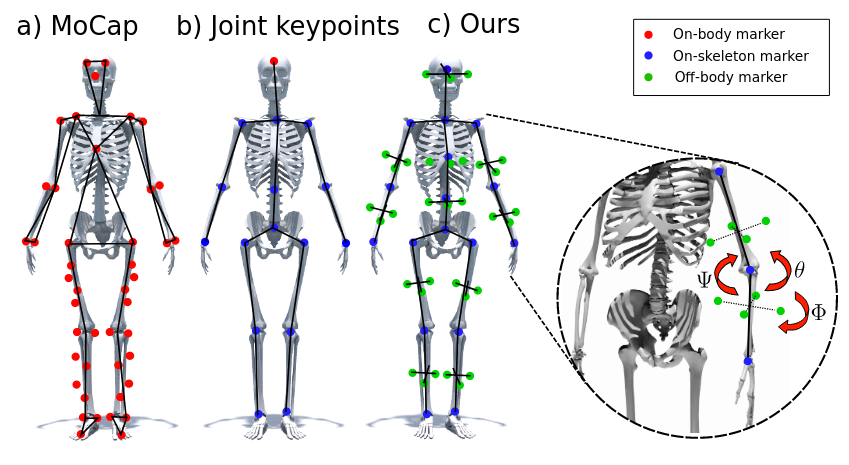
\includegraphics[width=0.8\linewidth]{figures/HPE/PoseExample.png}
    \caption{Example of a human pose captured with different methods. (a) A captured skeleton using MoCap which we do not focus on in this report. (b) A traditional human skeleton representation. (c) A pose representation that includes the orientation of the joints as well as the bones as presented by Martin Fish and Ronald Clark\cite{KeypointOrientation}}
    \label{fig:pose_example}
\end{figure}

The second way to visualise a human pose is by using a 2D silhouette or 2D rectangles and shapes. These methods are also called contour-based methods. An example of contour-based methods was introduced by Yunheng Liu\cite{contourHPE}. Contour-based methods are often used in combination with a skeleton representation. The skeleton is used to determine the location of the joints, while the contour is used to determine the shape of the body. This is useful when the skeleton is not able to determine the shape of the body, for example, when the person is wearing a coat or a jacket. This is also used for some games developed by SilverFit.

Finally, the third way to represent a human pose is with a three-dimensional volume. This volume may be simple cylindrical shapes or a body mesh. A body mesh is a 3D representation of the body, which is made up of vertices and triangles. The three different representations of the human pose can be seen in Figure \ref{fig:pose_representation}.

\begin{figure}
    \centering
    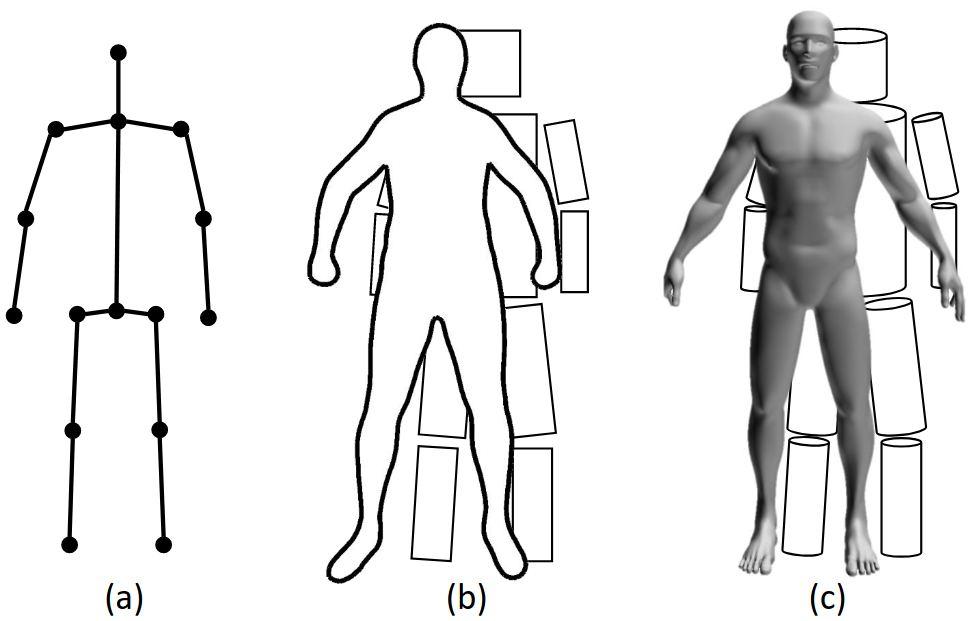
\includegraphics[width=0.8\linewidth]{figures/HPE/PoseRepresentation.png}
    \caption{Different representations of the human pose. (a) Skeleton representation. (b) Contour representation. (c) 3D volume representation. \cite{HPESurveyOriginal}}
    \label{fig:pose_representation}
\end{figure}

\subsection{Pose estimation data sources}

The pose of a human can be estimated from different types of data sources. The most common data source is RGB videos. RGB videos are any videos that are captured with normal cameras that record the color of the scene. The provided data can be either from a video or a stream of data or a still image. There is a large number of datasets that can be used to train and test pose estimation algorithms from RGB data. Some of the most common datasets are the MPII Human Pose Dataset\cite{MPII}, the COCO dataset\cite{Coco}, and HumanEva-I dataset\cite{HumanEva-I}.

Additionally, some datasets are captured with depth cameras. Depth cameras are cameras that can record the depth of the scene. This depth information can be used to improve the accuracy of the pose estimation. Some of the most common datasets that are captured with depth cameras are the MRI dataset\cite{mRI}, and the Human3.6M dataset\cite{h36m_pami}.

Finally, there are also methods of human pose estimation that use point clouds. Point clouds are a collection of points in space, which can be used to represent the shape of an object. Point clouds are often used in combination with RGB data. Some of the most common datasets that are captured with depth cameras are the SMMC-10 dataset\cite{SMMC10}, and the EVAL dataset\cite{EVAL}.

Additionally, to the data that is provided, we also differentiate between monocular and multi-modal data. Monocular data is data that is captured with a single camera. Multi-modal data is data that is captured with multiple cameras. The most common multi-modal data is stereo data, which is data that is captured with two cameras. The cameras are usually placed next to each other and are angled toward the same scene. This allows the cameras to capture the same scene from different angles and therefore improving the accuracy of the pose estimation. There are not many datasets for this type of data, but the most common one was captured by Waymo\cite{Waymo}.

However, RGB cameras are far more widely spread and generally cheaper than depth cameras. Hence, most methods use RGB cameras to estimate the pose of a human. However, since depth cameras can provide more detailed information about the scene, they can be used to improve the accuracy of the pose estimation and in this report, we will mainly focus on monocular RGBD data.

\subsection{Depth cameras}

As mentioned earlier, human pose estimation generally works based on visual information. However, the use of depth cameras offers more detailed information about the scene, which can in turn improve the reliability of the pose estimation. Many different depth cameras function mainly on three different principles. Firstly there are stereo cameras. Stereo cameras try to calculate the depth of a scene similar to how human eyes work. Most of the time two lenses or cameras are placed or installed next to each other and are angled toward the same scene and then the depth of the scene is calculated by comparing the images captured by the two cameras. These cameras function on the spectrum of light which is visible to the human eye. 

The second type of depth camera is the time-of-flight camera. These cameras use a laser to calculate the depth of the scene. The laser is fired at the objects in the scene, and the time it takes for the laser to bounce back is used to calculate the distance between the camera and the object based on the theoretical time it would take light to travel. 

Finally, there are also structured light cameras. These cameras use a pattern of light that is known to the camera to calculate the depth structure of the scene. For both the time-of-flight and structured light cameras, the depth information is calculated based on the spectrum of light that is not visible to the human eye.

\subsection{Applications}

Human pose estimation finds application in many different fields. Here we mention a few of the most common applications.

\subsubsection{Gaming and entertainment}

This is one of the most common applications of human pose estimation. Games can use human pose estimation in a way that makes the interaction between humans and computers very natural way.

\subsubsection{Autonomous Driving}

Autonomous driving has been in development ever since humans replaced horses with cars. However, the development of autonomous driving has been very slow. The main reason for this is that autonomous driving requires a lot of information about the environment. This information is usually provided by sensors that are installed in the car. However, sensors alone do not always suffice. In some cases, cars need to be able to estimate the pose of a human to make a decision. The posture of a human can be used to determine the action and therefore the future trajectory of the person. 

\subsubsection{Animation}

To emulate exactly human movements in animation, animators can either manually move the joints of a digital skeleton or they can use real human\footnote{Or animal} actors to provide the movement for them. The manual creation of realistic movement is oftentimes very time-consuming and also error-prone. Therefore, animators often use real human actors to provide the movement for them. This provides animators with a skeleton and movement which is accurate and does not include human error. In large production studios, this is often done with motion capture or MoCap. 

MoCap is a technique that uses cameras to capture the movement of a human actor. The cameras are placed around the actor and record the movement of the actor. The actor usually wears a suit that is covered with markers. These markers are used to determine the position of the actor. To reduce the amount of occlusion of the markers a large number of cameras are used. This allows the cameras to capture the movement of the actor from different angles. However, this also increases the price of development. In cases where MoCap is not a viable option, animators can use human pose estimation to estimate the pose of a human actor using cheaper RGB cameras or RGBD cameras.

\subsubsection{Healthcare}

One of the companies that develop games using human pose estimation is Silverfit. SilverFit uses both a skeletal representation as well as a contour representation of the human pose. 
\section{Research question}

As mentioned earlier, a major problem with human pose estimation is that it is not possible to tell if the joints are faulty or not. This is a problem for SilverFit, as they want to be able to tell if the joints are faulty or not. Using faulty joints can decrease the efficacy of the training effect of the developed games and can make them very frustrating to use and develop. A joint is considered faulty if it is not in the incorrect position, i.e. the distance from the theoretical position is greater than a chosen threshold, or if it missing from the skeleton.

In this thesis, we first ask what problems occur during human pose estimation and what common error sources are. We aim to find which problems are the most common and which joints are most affected by the errors. This will help give an overview of the issues related to human pose estimation and help develop ways to detect these issues. 

Once we know the issues that occur during human pose estimation, we aim to develop a method that can capture the camera stream in a way that allows us to label the data according to the exercise and environment it was captured in. This will allow us to create a dataset that can be used for future purposes.

Furthermore, we try to find if it is possible, given a joint, the RGB data, and the depth data, to determine if the joint is faulty or not.




\section{Process Pipeline}
\label{sec:process_pipeline}

The whole process of fault estimation can be seen as a pipeline. We start at the most basic starting block, the camera streams, and end at the most complex block, the fault estimation. The pipeline is shown in Figure \ref{fig:process_pipeline}. The pipeline consists of eight steps, which are described in more detail in the following sections. The steps are (\textbf{0}) Preliminary Analysis, (\textbf{I}) Stream Pre-Processing, (\textbf{II}) Data Acquisition, (\textbf{III}) Data Population, (\textbf{IV}) Data Post-Processing/Evaluation, (\textbf{V}) Data Augmentation, (\textbf{VI}) Model Training, and (\textbf{VII}) Model Evaluation. The results of each step are used as input for the next step. 

We further divided the process into a preliminary, data processing, and model development phase. The preliminary phase focuses on issue analysis and exercise development, the data processing phase is the first five steps of the pipeline. The model development phase is the last two steps of the pipeline.

In the next chapters, we give a basic overview of the whole process. We go into more detail in the following sections.

\begin{figure}[ht]
    \centering
    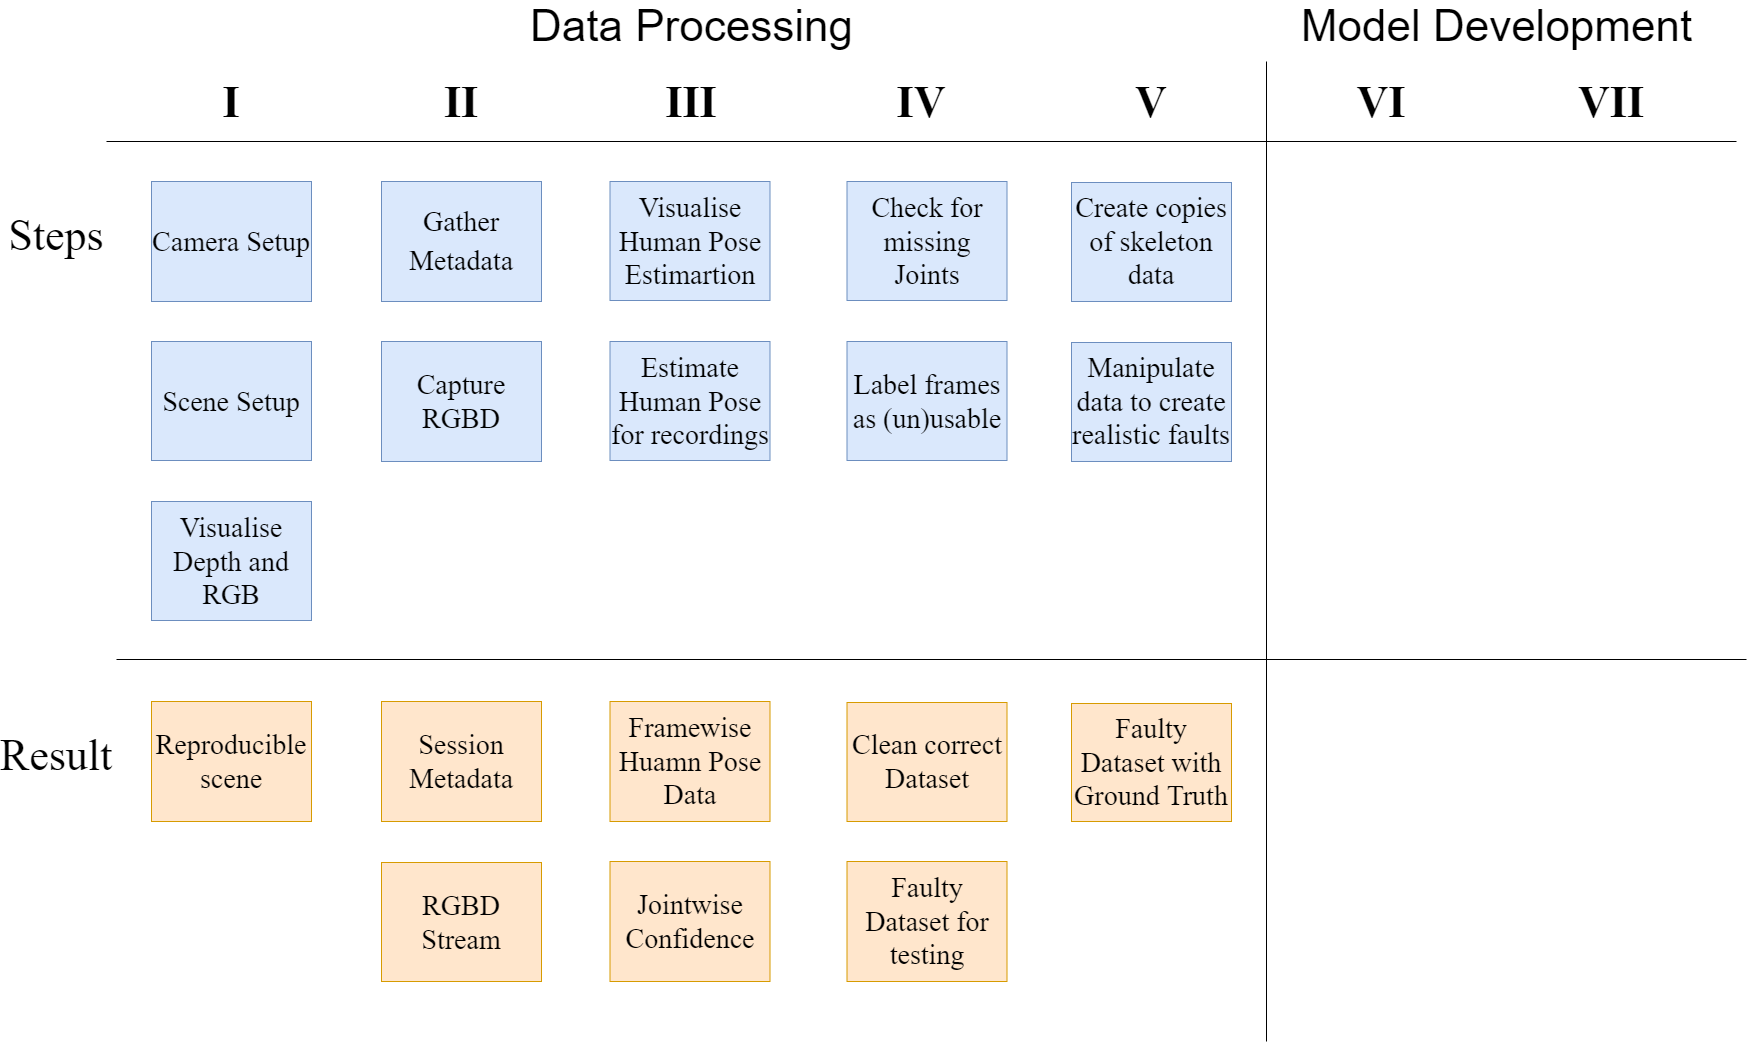
\includegraphics[width=\textwidth]{figures/ProcessingPipeline/ProcessingPipeline.png}
    \caption[Process Pipeline with all steps]{The whole Process pipeline with all the steps, which are marked in blue, and the results of each step, which are marked orange. The results of the steps are used as input for the next step. The steps are described in more detail in the following sections. The steps are: (\textbf{0}) Preliminary Analysis, (\textbf{I}) Stream Pre-Processing, (\textbf{II}) Data Acquisition, (\textbf{III}) Data Population, (\textbf{IV}) Data Post-Processing/Evaluation, (\textbf{V}) Data Augmentation, (\textbf{VI}) Model Training, and (\textbf{VII}) Model Evaluation.}
    \label{fig:process_pipeline}
\end{figure}

\section{Fundamentals}

In this section, $REPLACE_WE$ explain some of the fundamentals that are used during this thesis. 

\subsection{Human pose estimation}

There is wide variaty of how humans can interact with computers. Ranging from early punch cards to modern touch screens, the methods have evolved to be more natural and intuitive. In recent years, the use of cameras has become more popular, since they require no physical contact with a computer and therefore allow users to seamlessly interact with an application.

\subsubsection{Pose visualisation}

Different methods to capture the pose of a human have been developed. Depending on the usage of the pose estimation, different methods are used to visualise the pose of a human. These visualisations may provide different information about the pose of a human.

There are mainly three different ways the human pose can be visualised. The first and most basic way is to visualise the pose as a kinematic representation, in which a "skeleton" with bones and joints is used to represent the pose of a human. The skeleton is made up of joints, which are connected by bones. The number of joints and bones can vary, but the most common skeleton is made up of 17 joints and 16 bones, as can be seen in Figure \ref{fig:pose_example}. The joints are usually labeled with a number, which is used to identify the joint in the output of the pose estimation. The representation of a joint in the data varies, but it is usually a 2D or 3D point in space. In some cases, an additional joint representation is provided with a keypoint orientation that enables the clear representation of all degrees of freedoms joints have\cite{KeypointOrientation}. Additionally, in some cases, especially if the human pose was estimated using a neural network, a confidence rating or score is added which can be used to determine the reliability of the joint.

\begin{figure}
    \centering
    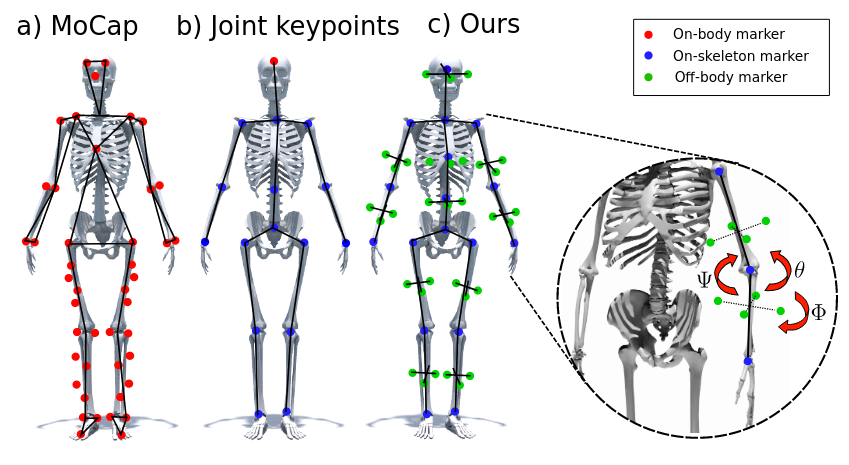
\includegraphics[width=0.8\linewidth]{figures/HPE/PoseExample.png}
    \caption[Example for human Pose estimation]{Example of a human pose captured with different methods. (a) A captured skeleton using MoCap which $REPLACE_WE$ do not focus on in this report. (b) A traditional human skeleton representation. (c) A pose representation that includes the orientation of the joints as well as the bones as presented by Martin Fish and Ronald Clark\cite{KeypointOrientation}}
    \label{fig:pose_example}
\end{figure}

The second way to visualise a human pose is by using a 2D silhouette or 2D rectangles and shapes. These methods are also called contour-based methods. An example of contour-based methods was introduced by Yunheng Liu\cite{contourHPE}. Contour-based methods are often used in combination with a skeleton representation. The skeleton is used to determine the location of the joints, while the contour is used to determine the shape of the body. This is useful when the skeleton is not able to determine the shape of the body, for example, when the person is wearing a coat or a jacket. This is also used for some games developed by SilverFit.

Finally, the third way to represent a human pose is with a three-dimensional volume. This volume may be simple cylindrical shapes or a body mesh. A body mesh is a 3D representation of the body, which is made up of vertices and triangles. The three different representations of the human pose can be seen in Figure \ref{fig:pose_representation}.

\begin{figure}
    \centering
    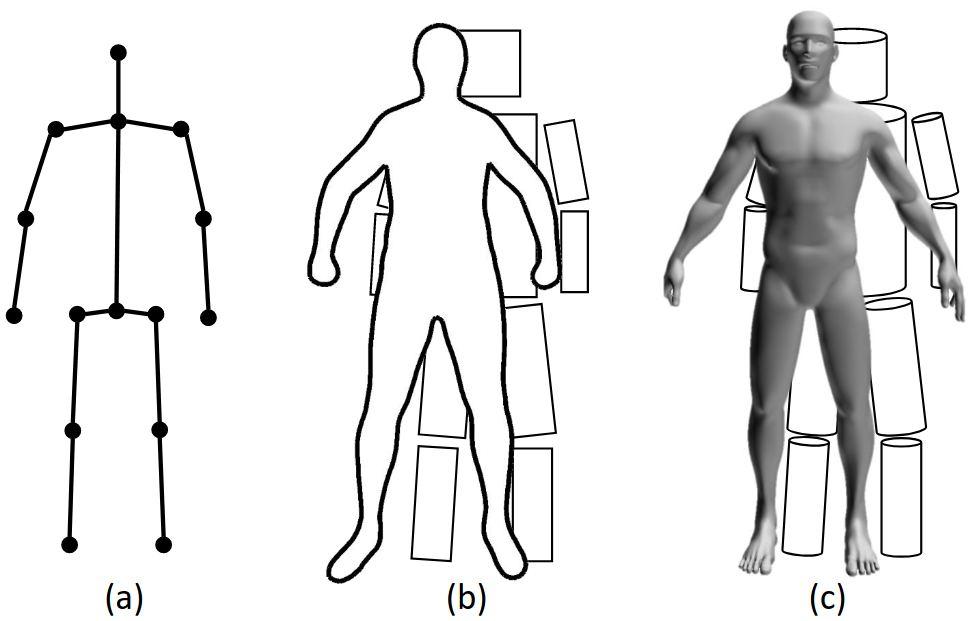
\includegraphics[width=0.8\linewidth]{figures/HPE/PoseRepresentation.png}
    \caption[Different representations of the human pose]{Different representations of the human pose. (a) Kinematic representation. (b) Contour representation. (c) 3D volume representation. \cite{HPESurveyOriginal}}
    \label{fig:pose_representation}
\end{figure}

\subsubsection{Data sources}

The data that is acquired influences the way the way the human pose can be estimated. The most common data source is RGB images or videos. RGB videos are any videos that are captured with normal cameras that record the color of the scene. The provided data can be either from a video or a stream of data or a still image. There is a large number of datasets that can be used to train and test pose estimation algorithms from RGB data. Some of the most common datasets are the MPII Human Pose Dataset\cite{MPII}, the COCO dataset\cite{Coco}, and HumanEva-I dataset\cite{HumanEva}.

Additionally, some datasets are captured with depth cameras. Depth cameras are cameras that can record, additionally to the color channels, the depth of the scene. Different methods to acquire depth data have been developed. The most commonly used depth cameras emitt an infrared light pattern to measure the depth of a scene. This depth information can be used to improve the accuracy of the pose estimation. Some of the most common datasets that are captured with depth cameras are the MRI dataset\cite{mRI}, and the Human3.6M dataset\cite{h36m_pami}.

Finally, there are also methods of human pose estimation that use point clouds. Point clouds are a collection of points in space, which can be used to represent the shape of an object. Each point in the point cloud represents a point in the environment. The point cloud is created using the depth information of a scene and the intrinsics of a camera, i.e. the field of view and the focal point of the camera. A point cloud is a reconstruction of the real world scene. Point clouds are often used in combination with RGB data. Some of the most common datasets that are captured with depth cameras are the SMMC-10 dataset\cite{SMMC10}, and the EVAL dataset\cite{EVAL}. However, any RGBD dataset can be used to train and test point cloud-based pose estimation algorithms if the camera intrinsics and extrinsic, such as the horizontal and vertical field of view, the focal point, and the depth units are known. With the knowledge of these parameters, the depth information can be converted to a point cloud and if the RGB data is in line with the depth data, the individual points can be coloured accordingly.

% \subsubsection{Depth cameras}

% Human pose estimation generally works based on visual information. However, the use of depth cameras offers more detailed information about the scene, which can in turn improve the reliability of the pose estimation. Many different depth cameras function mainly on three different principles. Firstly there are stereo cameras. Stereo cameras try to calculate the depth of a scene similar to how human eyes work. Most of the time two lenses or cameras are placed or installed next to each other and are angled toward the same scene and then the depth of the scene is calculated by comparing the images captured by the two cameras. These cameras function on the spectrum of light which is visible to the human eye. 

% The second type of depth camera is the time-of-flight camera. These cameras use a laser to calculate the depth of the scene. The laser is fired at the objects in the scene, and the time it takes for the laser to bounce back is used to calculate the distance between the camera and the object based on the theoretical time it would take light to travel. 

% Finally, there are also structured light cameras. These cameras use a pattern of light that is known to the camera to calculate the depth structure of the scene. For both the time-of-flight and structured light cameras, the depth information is calculated based on the spectrum of light that is not visible to the human eye.

\subsubsection{Applications}

Human pose estimation finds application in many different fields. Here $REPLACE_WE$ mention a few of the most common applications.

\paragraph{Gaming and entertainment}

One of the most common applications of human pose estimation. Games can use human pose estimation in a way that makes the interaction between humans and computers very natural way. One of the games that kickstarted the use of depth cameras in games was the game Kinect by Microsoft. This game used a depth camera to track the movement of the player and used this information to control the game. This game was very successful and was used in many different games. 

\paragraph{Autonomous Driving}

Autonomous driving has been in development ever since humans replaced horses with cars\cite{OldAutoDrive}. However, the development of autonomous driving has been very slow. The main reason for this is that autonomous driving requires a lot of information about the environment. This information is usually provided by sensors that are installed in the car. However, sensors alone do not always suffice. In some cases, cars need to be able to estimate the pose of a human to make a decision. The posture of a human can be used to determine the action and therefore the future trajectory of the person. 

\paragraph{Animation}

To exactly emulate human movements in animation, animators can either manually move the joints of a digital skeleton or they can use real human\footnote{Or animal} actors to provide the movement for them. The manual creation of realistic movement is oftentimes very time-consuming and also error-prone. Therefore, animators often use real human actors to provide the movement for them. This provides animators with a skeleton and movement which is accurate and does not include human error. In large production studios, this is often done with motion capture or MoCap. 

MoCap is a technique that uses cameras to capture the movement of a human actor. The cameras are placed around the actor and record the movement of the actor. The actor usually wears a suit that is covered with markers. These markers are used to determine the position of the actor. To reduce the amount of occlusion of the markers a large number of cameras are used. This allows the cameras to capture the movement of the actor from different angles. However, this also increases the price of development. In cases where MoCap is not a viable option, animators can use human pose estimation to estimate the pose of a human actor using cheaper RGB cameras or RGBD cameras.

\paragraph{Healthcare}

One of the companies that develop games using human pose estimation is Silverfit. SilverFit uses both a skeletal representation as well as a contour representation of the human pose. Human pose estimation enables the game to provide the user with feedback on their posture. This feedback can be used to improve the posture of the user and also allows the physiotherapists to design specific exercises which engage the muscles that are not used enough.

\subsection{Machine Learning}

\subsection{Evaluation metrics and mathematical formulas}

\subsubsection{Precision and Recall}

\subsubsection{F1-Score}

\subsubsection{Cross-Entropy Loss}
\section{Related Work}
\label{sec:related_work}

\textbf{This still needs a lot of work}


A plethora of methods have been developed to estimate the pose of a human. In this section, $REPLACE_WE$ will discuss some of the methods that have been developed to estimate the pose of a human. Additionally, $REPLACE_WE$ discuss datasets that have been developed to test the performance of the methods. Finally, $REPLACE_WE$ discuss some of the methods that have been developed to estimate the fault.

\subsection{Human Pose Estimation}


Human Pose Estimation using Iterative Error feedback. \cite{IterativeErrorFeedback}

While OpenPose developed Hand Pose\cite{OpenPoseHand} and also Multi-Person Human Pose Estimation \cite{OpenPoseMulti}, $REPLACE_OUR$ main focus lies on their most recent pose estimator \cite{OpenPosePose} and their CNN network \cite{OpenPoseCNN}. Openpose uses affinity fields. The affinity fields are a set of 2D Gaussian distributions that are used to estimate the pose of a human. The affinity fields are used to estimate the pose of a human by estimating the probability of a joint being in a certain location. The probability of a joint being in a certain location is calculated by summing the probability of the joint being in that location for each of the Gaussian distributions.

\subsubsection{Reviews}


A review of point cloud-based human pose estimation \cite{ReviewPointcloudHPE}

A review of 2D human pose estimation methods \cite{ReviewHPE}

\subsubsection{RGB Pose Estimation}

But $REPLACE_WE$ wont go into much detail as $REPLACE_WE$ focus on RGBD data.

\textbf{This is a bit wrong, the dataset is multi modal but the definition of multimodal is different in this method, it means RGB plus D and not different angles sometimes maybe not, read it through again:}
The limited number of multi-modal datasets causes the existence of human pose estimators for cameras from different angles to be small. One example of multi-modal human pose estimation was introduced by Jingxiao Zheng et al.\cite{MultiModalHPERGBD}. In their paper 

\subsubsection{RGBD Pose Estimation}

\textbf{This is a bit out of context:}
As mentioned by Jingxiao Zheng et al. in \cite{MultiModalHPERGBD}, the key points or joints of the skeleton do not lay on the surface of the person and therefore the determination of the exact position of the joints are not a direct projection on the depth image or the point cloud.

\cite{PASCUALHERNANDEZ2022102225}

\cite{RGBDHPEforRoboticTaskLearning}




\subsection{RGBD CNNs}

Early HPE algorithm uses trees \cite{EarlyRGBDHPE}

CNNs more useful for images and stuff. Cnns are not a new invention yada yada yada \cite{OldCNN}. But like many things in the neural network Biz, they were limited by the hardware available at the time. They have since formed the basis of many new methods in computer vision, such as Human Pose estimation. Especially AlexNet \cite{AlexNet} and VGG \cite{VGG} proved the potential of CNNs in Computer Vision tasks. 

\subsection{Object Detection}

\cite{Chen2021} Proposes different methods of fusion for RGBD data.

\subsubsection{Depth Completion}

Realsense with Tensorflow \cite{TensorflowRealsense} uses U-Net for depth completion \cite{UNET}.

\subsubsection{Action Recognition}

Cool CNN --> \cite{ElboushakiAbdessamad2020MAmf}

Another Review on human pose estimation but this time it is for action recognition \cite{ReviewHPEforActionRecognition}

In \cite{Seddik2017} Seddik et al. introduce different fusion methods for action recognition. They use RGB, Depth, and Skeleton data. After detecting the features for each modality, they fuse the features using different methods as can be seen in Figure \ref{fig:fusionmethods}. Seddik et al. use different bags of visual words (BoVW).

Human3.6M: Large Scale Datasets and Predictive Methods for 3D Human Sensing in Natural Environments \cite{h36m_pami}

Latent Structured Models for Human Pose Estimation \cite{IonescuSminchisescu11} 

\subsection{Anomaly Estimation}

This is quite close to my topic I will find some papers that do this and write about them.